\section{Evaluation}
\label{sec:evaluation}

\subsection{Method}
\label{sec:eval-method}

\paragraph{Pre-registration.}
We committed and tagged every hypothesis, decision rule and predicted
losing regime (\texttt{prereg-v1}) \emph{before} writing the simulator.
We did this because one author, working with a single AI model family
(Acknowledgments), produced \sys{}, the baselines and the simulator.
That is the main threat to validity~\cite{nosek2018prereg}.
After the tag, the plan changed only through dated, appended amendments
(A1--A11, Appendix~\ref{app:amendments}), and we report every hypothesis
whatever its outcome. Two amendments changed a decision and are disclosed
where they apply:
\begin{itemize}
\item \textbf{A4} repaired the weighting decision rule after we had seen
  plumbing-test numbers (\S\ref{sec:eval-trust}).
\item \textbf{A9}, requested by the author after an exploratory finding,
  re-chose the recommended weighting with a new rule. That rule was
  committed and pushed before its run.
\end{itemize}

\paragraph{Statistics.}
Each sweep point runs 20 seeds (60 for F1, matching its source). We report
means with 95\% percentile-bootstrap CIs over seeds (10,000
resamples~\cite{efron1993bootstrap}). A comparative hypothesis
\emph{holds at a point} only if the CI of the difference or ratio lies
entirely on the claimed side. Seeds are resampled jointly for paired
arms. We apply no multiple-comparison correction, and the full grid is
published.

\paragraph{Reproducibility.}
One command (\texttt{eval/run\_all.ps1}) builds the simulator, checks the
golden hashes, runs every experiment, and regenerates the report and the
figures. We ran the whole evaluation twice, at two commits:
\begin{itemize}
\item \textbf{Byte-identical outputs.} Every experiment that ran in both
  runs produced byte-identical CSVs.
\item \textbf{Run once.} The main trust grid ran only at the second
  commit, after a cache-blocking optimization verified to be bit-identical
  (A7). The two follow-up weighting sweeps (A8, A9) also ran once.
\item \textbf{Signing modes.} Real and fast signing produce identical
  output on a check grid, re-verified on every run (A1).
\end{itemize}

\begin{table}[t]
\caption{Pre-registered verdicts (20 seeds; F1: 60). ``Holds'' counts the
points whose 95\% CI lies on the claimed side. L1--L4 are
\emph{predicted} losing regimes, so ``occurs'' is a loss for \sys{}.}
\label{tab:verdicts}
\small
\begin{tabular}{@{}llr@{}}
\toprule
Id & Claim & Verdict \\
\midrule
F1-a & Replicates~\cite{wang2026agenticp2p} Fig.~5a within $\pm$0.05 & holds 12/12 \\
F1-b1 & At 60\,s, \sys{} adds nothing to Risk-Aware & partial 5/6 \\
F1-b2 & At 3600\,s, \sys{}+RA $-$ RA $\ge 0.10$ & holds 4/4 \\
F1-b3 & \ldots\ under 60\,s whitewashing, $\ge 0.05$ & holds 2/2 \\
H1 & Attacker share $\le 0.5\times$ B1 and B2 & \textbf{partial 18/28} \\
L1 & Cold start: worse than B2, rounds 1--5 & occurs 35/35 \\
L2 & Sparse evidence: W0 $\not<$ random & did not occur \\
L3 & On-off: decay lags the off phase & occurs 5/5 \\
L4 & Camouflage hurts W1/W2 ($\alpha{=}0.2$) & did not occur \\
H2 & Resume waste $\le 0.4\times$ restart & holds \\
H3 & D-6 caps flooding at fair share & holds 6/6 \\
H4 & Pulled status beats descriptor-carried & holds 4/4 \\
H5 & Exposure $\le$ price($c$); CPU overhead $<$1\% & holds 6/6 \\
\bottomrule
\end{tabular}
\end{table}

\subsection{Replicating an agentic P2P baseline}
\label{sec:eval-f1}
Before comparing against Wang et al.'s Risk-Aware
policy~\cite{wang2026agenticp2p}, we re-implemented their simulator's model
from its source code. We read that code but did not execute it. The model:
\begin{itemize}
\item 100 peers, a fraction $\alpha$ of them Sybils that overclaim their
  self-reported hints and succeed 5\% of the time;
\item two-step workflows, a shortlist of 25, and up to three attempts
  per step;
\item a canary that honest peers pass 97\% of the time and Sybils 8\%.
\end{itemize}
Our curves match their published Fig.~5a at all 12 points to within
$\pm$0.05; the largest difference is 0.024 (Figure~\ref{fig:f1}). This
gate had to pass before any comparison.

We then added \sys{}'s local projection, evaluated in their world:
\begin{itemize}
\item \textbf{Short horizon.} In their 60\,s horizon, a requester has
  less than one workflow of its own history. As predicted, \sys{}
  ranking in front of the canary (\sys{}+RA) adds nothing at five of six
  values of $\alpha$. The exception is $\alpha{=}0.3$, a small gain of
  $+0.037$\ci{0.002}{0.071}.
\item \textbf{One hour.} At 3,600\,s, evidence accumulates and \sys{}+RA
  beats Risk-Aware by 0.123 to 0.265 for $\alpha\in[0.2,0.5]$.
\item \textbf{Whitewashing.} With Sybils re-keying every 60\,s, it still
  beats Risk-Aware by 0.105 at $\alpha{=}0.2$ and 0.169 at
  $\alpha{=}0.3$, because honest providers keep their history.
\end{itemize}
Risk-Aware verifies each task; it does not remember the result. \sys{}
supplies the memory.

\begin{figure}[t]
  \centering
  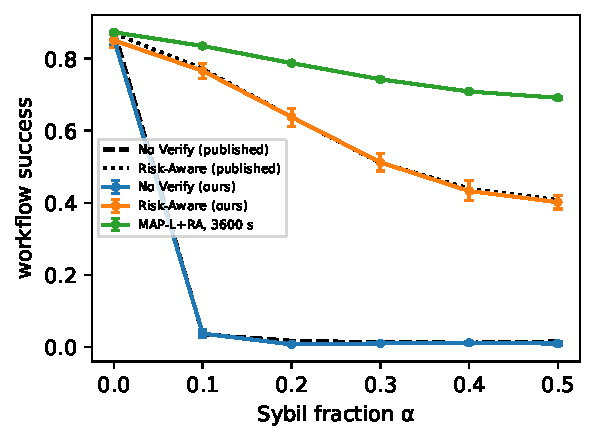
\includegraphics[width=0.9\columnwidth]{figs/f1_replication}
  \caption{Replication of~\cite{wang2026agenticp2p} Fig.~5a (dashed:
  published; solid: ours, 60 seeds, 95\% CIs) and \sys{}'s local
  projection with the canary over a 3,600\,s horizon.}
  \label{fig:f1}
\end{figure}

\subsection{Trust under attack (E1)}
\label{sec:eval-trust}

\paragraph{World.}
The simulated world has:
\begin{itemize}
\item 200 providers and 500 honest requesters over 60 rounds; one round
  is one day of decay;
\item Poisson(2) tasks per requester per round;
\item a shortlist of 10 providers per task, with 10\% uniform
  exploration and up to 3 attempts.
\end{itemize}
Honest providers succeed with $q\sim U[0.80,0.98]$. A fraction $\alpha$
of providers is adversarial, with $q{=}0.2$. Adversarial providers refuse
to countersign their failures. In the Sybil attacks (farming, camouflage,
slander, combined), each one also controls 20 Sybil requesters.
Every receipt goes to one public pool, the worst case. Discovery is
honest: shortlists are drawn from the real providers only
(\S\ref{sec:eval-discovery} drops this assumption). The metric is the
steady-state (rounds 31--60) share of honest requesters' tasks that go to
adversarial providers.

\paragraph{Arms.}
\begin{itemize}
\item \textbf{B0}: random selection.
\item \textbf{B1}: a global ledger in the style of ERC-8004. It is
  \sys{}'s own projection with every issuer weighted~1; it keeps the
  decay and the cap, which makes it a \emph{stronger} baseline than a raw
  sum (A3).
\item \textbf{B2}: Risk-Aware's canary.
\item \textbf{B2L}: B2 plus a ledger of provider-signed receipts, the
  paper's prose design.
\item \textbf{Ours-L}: \sys{}.
\item \textbf{Ours-L+C}: \sys{} with the canary in front.
\item \textbf{Ablations:} unknown issuers weighted 0.5
  (\emph{A-prior}); requester-only positive receipts admitted
  (\emph{A-unilateral}).
\end{itemize}

\begin{figure*}[t]
  \centering
  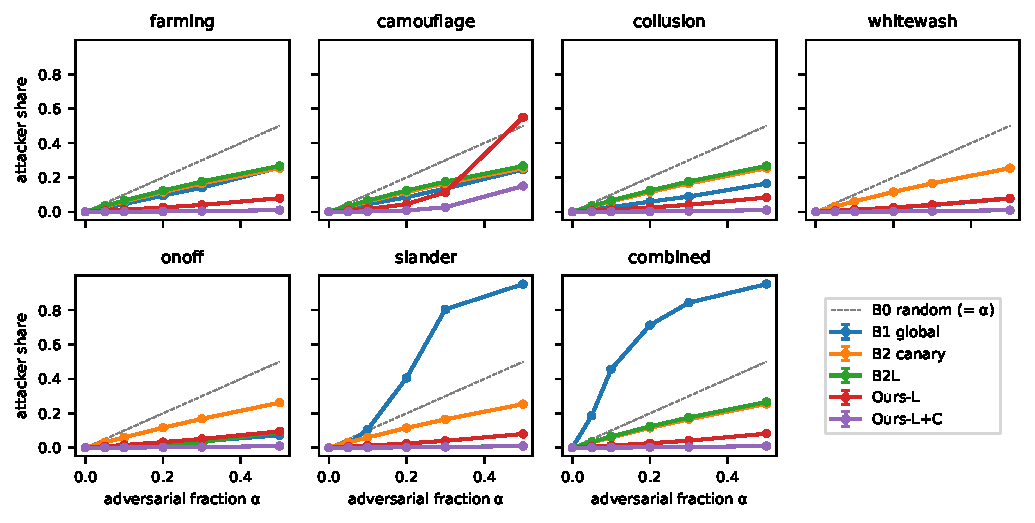
\includegraphics[width=\textwidth]{figs/e1_attacker_share}
  \caption{E1: steady-state attacker share of honest requesters' tasks
  versus adversarial fraction $\alpha$ (20 seeds, 95\% CIs). The dashed
  line is random selection. Ours-L uses the pre-registered weighting, W2;
  Table~\ref{tab:w1h1} gives the recommended W1.}
  \label{fig:e1}
\end{figure*}

\paragraph{Results (Figure~\ref{fig:e1}).}
H1 is only \textbf{partially} supported: Ours-L's attacker share is at
most half of both baselines' at 18 of 28 points. Against the canary
baseline B2 it holds at 27 of 28 points. The exception is camouflage at
$\alpha{=}0.3$, with a ratio of 0.69. Against the global ledger B1, H1
fails in three families:
\begin{itemize}
\item \textbf{Whitewashing.} The ratio is about 1.04 at every $\alpha$.
  Fresh identities have no evidence under \emph{either} scheme, so both
  sit at the floor set by exploration and fallback. Halving that floor
  is not possible.
\item \textbf{On-off.} The ratio is about 1.4. B1 pools every issuer's
  evidence, so it sees the ``off'' phase sooner than an observer that
  trusts only issuers resembling itself.
\item \textbf{Camouflage at $\alpha\ge0.2$.} Discussed below.
\end{itemize}
In the other direction, the global ledger \emph{collapses} under slander:
\begin{itemize}
\item B1's attacker share is 0.406 at $\alpha{=}0.2$ and 0.952 at
  $\alpha{=}0.5$. Sybil complaints bury honest providers, and the
  adversaries inherit the traffic.
\item Ours-L stays at 0.025 and 0.080, because complaints from issuers
  that disagree with the observer weigh nothing.
\item Under combined attacks B1 reaches 0.713 at $\alpha{=}0.2$.
\end{itemize}
\paragraph{Ablations.}
A-prior confirms T-3. With unknown issuers weighted 0.5 (the v1 design),
farming wins 0.715 of tasks at $\alpha{=}0.2$; with weight 0 it wins
0.025.

A-unilateral does \emph{not} test R-4, and we do not claim it does. In
E1 no agent emits a receipt that R-4 would stop from counting as
positive evidence:
\begin{itemize}
\item honest successes are dual-signed;
\item farming is dual-signed too, because the attacker holds both keys;
\item the only single-signed receipts are negative ones.
\end{itemize}
The arm therefore admits a receipt type that never occurs, and its
attacker share differs from Ours-L's by at most 0.0023 in any cell. That
difference is noise between independent random streams. What E1 measures
is issuer weighting (T-3). R-4's protection against a lone provider
minting its own praise (G1) is argued in \S\ref{sec:security}, not
measured.

\paragraph{The canary and Wang et al.'s full design.}
The canary composes with \sys{}: Ours-L+C keeps the attacker share at or
below 0.15 in every cell, and at or below 0.004 in every cell with
$\alpha\le0.3$ except camouflage.

B2L, the canary plus a provider-signed ledger, is the design Wang et al.'s
prose describes, and Figure~\ref{fig:e1} plots it. H1 did not
pre-register a comparison with it, so the one below is exploratory
(Table~\ref{tab:b2l}). The arms do not share random streams, so each is
resampled independently.
\begin{itemize}
\item \textbf{Ours-L+C against B2L.} Across all 35 cells, Ours-L+C is
  lower in 25 and never higher. It is lower in every cell under farming,
  camouflage, collusion, on-off and combined attacks, and the CIs overlap
  in the other ten (whitewashing and slander).
\item \textbf{Ours-L alone against B2L.} Without a canary, Ours-L is
  higher than B2L under whitewashing and slander at every $\alpha$, and
  under on-off at four of five. B2L's canary catches fresh identities,
  and its ledger admits only provider-signed receipts, so Sybil
  complaints never reach it.
\item \textbf{Where B2L is weak.} B2L's ledger is open to farming: at
  $\alpha{=}0.2$ it gives adversaries 0.123 of tasks, against 0.025 for
  Ours-L and 0.002 for Ours-L+C.
\end{itemize}

\begin{table}[t]
\caption{Exploratory: B2L (canary + provider-signed ledger) against
\sys{}, steady-state attacker share at $\alpha{=}0.2$, W2 weighting
(20 seeds; every 95\% CI is within $\pm$0.004 of the mean). All 35 cells
are in \texttt{B2L.md}.}
\label{tab:b2l}
\small
\begin{tabular}{@{}lrrr@{}}
\toprule
Attack & B2L & Ours-L & Ours-L+C \\
\midrule
farming & 0.123 & 0.025 & 0.002 \\
camouflage & 0.124 & 0.045 & 0.008 \\
collusion & 0.124 & 0.025 & 0.002 \\
whitewash & 0.002 & 0.025 & 0.002 \\
on-off & 0.018 & 0.033 & 0.002 \\
slander & 0.002 & 0.025 & 0.002 \\
combined & 0.124 & 0.026 & 0.002 \\
\bottomrule
\end{tabular}
\end{table}

\paragraph{Losing regimes.}
All four predicted losing regimes were tested:
\begin{itemize}
\item \textbf{Cold start (L1): occurs everywhere.} In rounds 1--5,
  Ours-L without the canary has a higher attacker share than B2: by
  0.014 at $\alpha{=}0.05$, up to 0.217 at $\alpha{=}0.5$. Local trust
  needs history, and a deployment should run a canary until it has some.
\item \textbf{On-off (L3): occurs.} At the start of each off phase the
  attacker share exceeds steady state by 0.017 to 0.196, the lag of a
  0.98/day decay.
\item \textbf{Sparse evidence (L2): did not occur.} At 0.1 tasks per
  requester per round, self-only weighting still beat random, by 0.9 to
  2.3 points.
\item \textbf{Camouflage (L4): did not occur at the pre-registered
  $\alpha{=}0.2$.} Agreement-based weights were not worse than self-only
  there. At higher $\alpha$ they were, as described next.
\end{itemize}

\paragraph{Detection time and whole-run share.}
Two further pre-registered E1 metrics are in \texttt{PREREG-EXTRA.md}.
\emph{Time to detect} is the first round from which the attacker share,
averaged over five rounds, is at most $\alpha/4$.
\begin{itemize}
\item \textbf{Ours-L} reaches $\alpha/4$ after 26--33 rounds with W2 and
  27--38 with W1 in 34 of 35 cells. It never does under camouflage at
  $\alpha{=}0.5$.
\item \textbf{The canary alone (B2)} never reaches it in any cell: it
  holds the attacker to $0.51$--$0.62\alpha$.
\item \textbf{B1} never reaches it in 18 of 35 cells, and \textbf{B2L}
  in 20.
\item \textbf{Ours-L+C} is below it from the first round in every cell.
\end{itemize}
Over all 60 rounds, which include the cold start, Ours-L's attacker share
is about three times its steady-state value (0.076 against 0.025 at
$\alpha{=}0.2$ under farming). Ours-L+C stays at or below 0.023 for
$\alpha\le0.3$ and reaches at most 0.098 at $\alpha{=}0.5$.

\paragraph{Choosing the weighting: a pre-registered rule, a collapse,
and a re-test.}
The pre-registered rule compared W0/W1/W2 at $\alpha{=}0.2$ only.
Averaged over all attacks, the steady-state attacker shares were:
\begin{itemize}
\item W0: 0.0796;
\item W1: 0.0312;
\item W2: 0.0290.
\end{itemize}
It selected W2 (A6). One disclosure applies: the rule's tie clause, as
first written, was satisfied almost always, and it would have chosen W0.
We repaired it (A4) \emph{after} seeing two-seed plumbing numbers, and
report both readings.

The main grid then showed W2 \emph{worse than random} under camouflage
at $\alpha{=}0.5$: 0.550, against 0.500 for random selection. At that
point 2,000 camouflaging Sybils face 500 honest requesters. Their
truthful reports about honest providers earn them agreement edges, and
propagation concentrates the observer's trust mass in the Sybil cluster.
This is the classic weakness of transitive trust against Sybils who have
bought honest-looking edges~\cite{yu2006sybilguard,cheng2005sybilproof}.
We had not tested it at that $\alpha$.

An exploratory run confirmed the collapse and showed that W1 does not
suffer it (A8). We then pre-registered a minimax rule (A9) and pushed it
before its run: choose the weighting with the lowest worst-case attacker
share over all 35 ($\alpha$, attack) cells. Table~\ref{tab:minimax}
gives the worst cells; Figure~\ref{fig:minimax} shows the two families
where the weightings differ most.

W1 wins, with non-overlapping CIs, and the specification recommends it.
The price is small. Outside on-off and camouflage, W2 is ahead by at most
0.003 at $\alpha\le0.3$ and by at most 0.007 at $\alpha{=}0.5$. Under
on-off it is ahead by 0.003 to 0.040. H1 and the other E1
verdicts stay as pre-registered, computed with W2.

\paragraph{H1 for the recommended weighting (exploratory).}
Every E1 headline above uses W2, which the specification no longer
recommends. Table~\ref{tab:w1h1} applies the H1 criterion to W1 instead.
W1's cells come from a separate run with independent random streams, so
each ratio's CI resamples the two arms independently. W2 is recomputed
the same way. That reproduces its pre-registered counts exactly: 18 of
28 points, and 27 of 28 against B2 alone.
\begin{itemize}
\item \textbf{Overall.} With W1, H1 holds at 17 of 28 points, and
  against the canary alone at all 28.
\item \textbf{Where W1 differs from W2.} It passes camouflage against B2
  at $\alpha{=}0.3$, with a ratio of 0.44 where W2 had 0.69. It fails
  collusion at $\alpha{=}0.3$, with a ratio of 0.49 whose upper bound is
  0.51. Both calls turn on margins of about 0.01.
\item \textbf{Against the global ledger under on-off} W1 is further
  behind than W2: a ratio of 1.85--1.94, against about 1.4.
\item \textbf{The slander result holds for W1:} 0.027 at $\alpha{=}0.2$
  and 0.084 at $\alpha{=}0.5$, against B1's 0.406 and 0.952.
\end{itemize}

\begin{table}[t]
\caption{Exploratory: the H1 criterion (Ours-L at most half of both B1
and B2, upper CI $\le$ 0.5) for W2 and W1, per attack, over the
pre-registered $\alpha\in\{0.05,0.1,0.2,0.3\}$. The arms are resampled
independently. The ratio columns give W1's range of point estimates over
$\alpha$. All cells are in \texttt{W1-H1.md}.}
\label{tab:w1h1}
\small
\begin{tabular}{@{}lrrrr@{}}
\toprule
Attack & W2 holds & W1 holds & W1/B1 & W1/B2 \\
\midrule
farming & 4/4 & 4/4 & 0.28--0.31 & 0.20--0.26 \\
camouflage & 2/4 & 2/4 & 0.40--0.53 & 0.28--0.44 \\
collusion & 4/4 & 3/4 & 0.45--0.49 & 0.20--0.26 \\
whitewash & 0/4 & 0/4 & 1.05--1.08 & 0.19--0.25 \\
on-off & 0/4 & 0/4 & 1.85--1.94 & 0.34--0.41 \\
slander & 4/4 & 4/4 & 0.05--0.24 & 0.20--0.26 \\
combined & 4/4 & 4/4 & 0.03--0.05 & 0.19--0.26 \\
\midrule
total & 18/28 & 17/28 & & \\
\bottomrule
\end{tabular}
\end{table}

\paragraph{Sybil count (exploratory, A10).}
E1 fixes 20 Sybil requesters per adversarial provider. Identities are
free, though, and W1 weights each camouflaging Sybil by its own agreement
with the observer, so nothing bounds how many count. Amendment A10,
pushed before its run, sweeps that number at $\alpha{=}0.2$
(Table~\ref{tab:sybils}):
\begin{itemize}
\item W1 held at 5 and 20 Sybils per provider, which is 0.4 and 1.6 per
  honest requester.
\item At 80, or 6.4 per honest requester, it lost to self-only weighting:
  0.077 against 0.072. At 320 it reached 0.165. It never became worse
  than random (0.2).
\item W2 was worse than random at 320 (0.526), even at $\alpha{=}0.2$.
\item Farming without camouflage stayed flat at every count, so the
  damage comes from bought agreement.
\end{itemize}
The attack is not cheap. Each camouflaging Sybil runs two real tasks per
round, so at 80 Sybils per provider the attacker buys 6.4 times the
honest workload. W1's minimax win therefore holds at the Sybil ratio of
the main grid, not in general, and the specification now says so.

\begin{table}[t]
\caption{Exploratory (A10): steady-state attacker share under camouflage
at $\alpha{=}0.2$ versus Sybils per adversarial provider (20 seeds; every
95\% CI is within $\pm$0.004 of the mean). ``Bought'' is the camouflage
tasks per round as a multiple of the honest workload. Random selection
gives 0.2.}
\label{tab:sybils}
\small
\begin{tabular}{@{}rrrrrr@{}}
\toprule
Sybils/prov. & Sybils/honest & Bought & W0 & W1 & W2 \\
\midrule
5 & 0.4 & 0.4$\times$ & 0.073 & 0.031 & 0.027 \\
20 & 1.6 & 1.6$\times$ & 0.072 & 0.041 & 0.045 \\
80 & 6.4 & 6.4$\times$ & 0.072 & 0.077 & 0.196 \\
320 & 25.6 & 25.6$\times$ & 0.072 & 0.165 & 0.526 \\
\bottomrule
\end{tabular}
\end{table}

\begin{table}[t]
\caption{A9 minimax re-test: each weighting's worst cell over
$\alpha\in\{0.05,\ldots,0.5\}\times$ seven attacks (steady-state attacker
share, 95\% CI).}
\label{tab:minimax}
\small
\begin{tabular}{@{}llll@{}}
\toprule
Weighting & Worst cell & Attacker share & Honest succ. \\
\midrule
W0 self only & 0.5, on-off & 0.348\ci{0.346}{0.350} & 0.960 \\
\textbf{W1 direct} & 0.5, camouflage & \textbf{0.200}\ci{0.196}{0.204} & 0.978 \\
W2 propagation & 0.5, camouflage & 0.550\ci{0.543}{0.557} & 0.867 \\
\bottomrule
\end{tabular}
\end{table}

\begin{figure}[t]
  \centering
  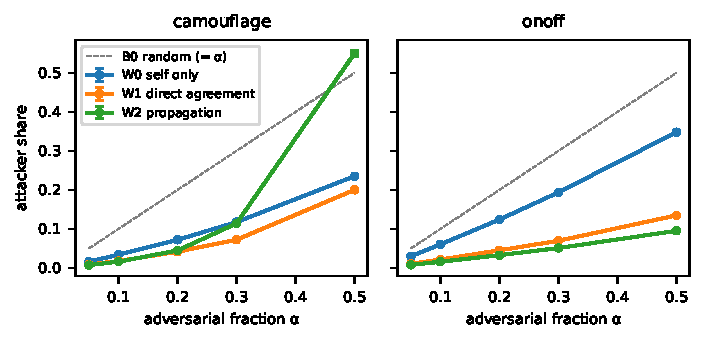
\includegraphics[width=\columnwidth]{figs/e1_minimax}
  \caption{Issuer weightings under camouflage and on-off (20 seeds, 95\%
  CIs). W2's propagation collapses once camouflaging Sybils outnumber
  honest requesters. W1 never does worse than random at the 20 Sybils per
  adversarial provider used here; Table~\ref{tab:sybils} varies that.}
  \label{fig:minimax}
\end{figure}

\subsection{Countersigned resumption (E2)}
\label{sec:eval-checkpoint}
Tasks of $L\in\{10^2,10^3,10^4\}$ Parts fail with hazard $\lambda$, with
$\lambda L\in\{0.1,1,3\}$ expected failures per task, and are resumed on
a fresh provider. We compare three recovery strategies: restarting from
scratch; resuming from a countersigned checkpoint every $c$ Parts; and
resuming from the failed provider's own claim of progress (provider-only).

\begin{itemize}
\item \textbf{H2 holds.} At $L{=}10^3$, $\lambda L{=}1$, $c{=}8$:
  \begin{itemize}
  \item countersigned resumption wastes 3.2\ci{2.8}{3.7} Parts per task;
  \item restarting wastes 768.6\ci{655.1}{881.7};
  \item the ratio is 0.0042\ci{0.0036}{0.0050}.
  \end{itemize}
\item \textbf{The billing rule (C-5) holds by construction.} The
  simulator bills a failed provider exactly its acknowledged usage.
  Its check that no run bills more than was delivered is therefore an
  invariant, not evidence. What C-5 costs is the provider's unpaid work,
  the Parts delivered after its last checkpoint. That is fewer than $c$
  per failure because the provider checkpoints every $c$ Parts. At the
  H2 operating point it averages 3.2 Parts per task. Under countersigned
  resumption, the waste above is exactly this unpaid work.
\item \textbf{Provider-only resumption} wastes nothing, whether or not
  providers are honest. With 20\% dishonest providers who overstate
  progress by 50\%, it overbills requesters by 30.2\ci{20.5}{41.3}
  Parts per task at the H2 operating point. It also causes
  0.20\ci{0.15}{0.27} transcript-integrity failures per task. At
  $\lambda L{=}3$ the figures are 53.0\ci{40.8}{66.0} and 0.45.
  Countersigned resumption has neither.
\end{itemize}

\paragraph{What H2 does and does not show.}
H2 compares countersigned resumption with restarting. Its saving belongs
to \emph{checkpointing}, not to countersigning: provider-only resumption
checkpoints too, and it wastes nothing. What countersigning buys is
safety. A dishonest provider cannot overbill, and a successor never
inherits a transcript the requester did not verify. That result follows
from the adversary model by construction, so E2 illustrates it; it does
not measure it. The measured claim is narrower: checkpointed resumption
regenerates 0.42\% of what restarting does, and countersigning adds its
safety at the cost of two signatures per checkpoint (\S\ref{sec:eval-meter}).
\paragraph{What the waste metric counts.}
E2's waste counts regenerated Parts. It does not count the successor's
cost to fetch, verify and ingest the replayed prefix. Verifying is cheap:
recomputing the root costs about $1.3\,\mu$s per Part. Ingesting is not
free. Failures arrive at rate $\lambda$ per Part of progress, and
resumption loses no progress, so the expected prefix replayed per task is
$\lambda L^2/2$. That is about 500 Parts at the H2 operating point,
against 3.2 regenerated. If ingesting a Part costs a fraction $\rho$ of
generating one, resumption costs about $3.2+500\rho$ Parts against
restart's 768.6. H2's conclusion therefore survives for any $\rho$ below
about 1.5. For language models, prefill is usually much cheaper per token
than decoding. The 0.42\% figure, however, compares regeneration only.
The specification defers an engine-state fast path that would let a
compatible successor skip ingestion. Resumption is always by transcript
replay.

Figure~\ref{fig:e2} shows the trade-off in $c$: waste grows roughly
linearly in $c$, while signatures shrink as $1/c$. Pricing a signature at
$\kappa\in\{0.01,0.1\}$ Parts of work, most settings are optimized
between $c{=}8$ and $c{=}32$. Those prices count signing only. When the
provider pauses for each countersignature, a checkpoint also costs a
round trip, and $\kappa$ rises to 1.25--2.5 per signature (\S\ref{sec:eval-meter}).
At $\kappa{=}1$ the optimum is $c{=}32$ at the H2 operating point, and
32--128 in 8 of 9 settings. The default (C-6) is therefore $c{=}8$ when
countersignatures are asynchronous and $c{=}32$ when they pause the task.

\begin{figure}[t]
  \centering
  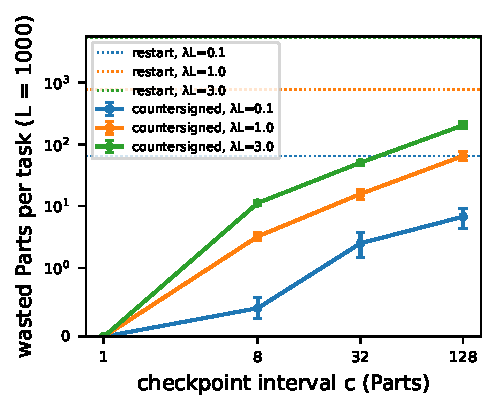
\includegraphics[width=0.85\columnwidth]{figs/e2_waste}
  \caption{E2 ($L{=}1000$): wasted Parts per task under countersigned
  resumption versus checkpoint interval $c$. Dotted lines: restart from
  scratch, in the same colour as the $\lambda L$ they match. At $c{=}1$
  no work is wasted.}
  \label{fig:e2}
\end{figure}

\subsection{Discovery (E3)}
\label{sec:eval-discovery}
\paragraph{Shard flooding (H3).}
An attacker holding a fraction $a$ of identities publishes its records
into every shard that queriers sample:
\begin{itemize}
\item \textbf{Without D-6}, it holds 46--91\% of candidates for
  $a\in\{0.01,0.05,0.1\}$.
\item \textbf{With D-6's shard check}, its share equals $a$ within 0.01
  at all six points ($n\in\{10^3,10^4\}$).
\end{itemize}

\paragraph{Identifier grinding: no mitigation.}
Generating a key pair and computing its shard costs 16.4\,$\mu$s on one
core, so an attacker makes 60,901 attempts per second.
\begin{itemize}
\item \textbf{Result.} Epoch-salted shard assignment, which re-randomizes
  every agent's shard each epoch, did not help: the attacker held
  1.000\ci{1.000}{1.000} of the target shard in all 27 configurations
  (network size, attack window, and epoch length).
\item \textbf{Why.} One core adds about 238 identities per second to any
  shard, while a shard of a $10^5$-provider network holds about 390
  honest providers. The attacker therefore has a majority about 2\,s
  after each re-salt.
\end{itemize}
A 16-core attacker, the exploratory variant of Amendment A5, also holds
the whole target shard in every configuration. When identities are free,
grinding is just targeted Sybil creation, and no shard function prevents
it. The specification now says so plainly (\S\ref{sec:security}).

\paragraph{Flooded discovery composed with trust (exploratory, A11).}
E1 assumes honest discovery, while E3b shows that discovery can be
flooded cheaply. Amendment A11, pushed before its run, composes the two.
Discovery returns $F$ zero-evidence adversarial identities alongside the
200 real providers, and every shortlist is drawn from both. It also
tests one local policy: \emph{shortlist memory}, where $k$ slots hold the
requester's best-scored providers among those it has a success receipt
for. Table~\ref{tab:flood} gives the results at $\alpha{=}0.2$ under
farming, with W1.
\begin{itemize}
\item \textbf{Without memory, trust cannot help once the flood is
  heavy.} At 10 flood identities per honest provider, discovery returns
  adversaries 91\% of the time, and Ours-L gives them 0.888 of tasks.
  Ranking cannot pick a provider that discovery never showed.
\item \textbf{Memory and the canary together protect established
  requesters.} With $k{=}3$, Ours-L+C holds the attacker to 0.036 at 10
  flood identities per honest provider and to 0.085 at 100. Honest
  success stays at 0.94 or above.
\item \textbf{New requesters are not protected.} In rounds 1--5 they have
  no memory, and Ours-L+C with $k{=}3$ still gives adversaries 0.182 and
  0.660 of tasks.
\end{itemize}
So E1's results hold only while discovery keeps returning honest
candidates. Discovery capture, not grinding into one shard, is the main
open problem.

\begin{table}[t]
\caption{Exploratory (A11): steady-state attacker share with a flooded
discovery layer ($\alpha{=}0.2$, farming, W1, 20 seeds; every 95\% CI is
within $\pm$0.008 of the mean). ``Disc.'' is the adversarial share of
discovery, which is also random selection's share. $k$ is the shortlist
memory. ``New'' is rounds 1--5.}
\label{tab:flood}
\small
\begin{tabular}{@{}rrrrrrr@{}}
\toprule
 & & \multicolumn{2}{c}{Ours-L} & \multicolumn{3}{c}{Ours-L+C} \\
Flood & Disc. & $k{=}0$ & $k{=}3$ & $k{=}0$ & $k{=}3$ & new, $k{=}3$ \\
\midrule
0 & 0.20 & 0.027 & 0.024 & 0.002 & 0.002 & 0.007 \\
1 & 0.56 & 0.211 & 0.086 & 0.023 & 0.010 & 0.032 \\
10 & 0.91 & 0.888 & 0.199 & 0.435 & 0.036 & 0.182 \\
100 & 0.99 & 0.990 & 0.634 & 0.892 & 0.085 & 0.660 \\
\bottomrule
\end{tabular}
\end{table}

\paragraph{Eclipse (E3c).}
In a simulated Kademlia (20-entry buckets, 3 parallel queries) with a
fraction $f$ of malicious routers, three disjoint lookup paths raise
lookup success at $N{=}10^5$ with $f{=}0.3$ from 0.755 to 0.930 without
churn, and from 0.906 to 0.975 with 10\% churn (Figure~\ref{fig:e3c}).
They cost 1.3--1.7$\times$ the messages. This
replicates the S/Kademlia result~\cite{baumgart2007skademlia}, and D-9
became a SHOULD.

\paragraph{Volatile plane (H4).}
Queue lengths follow an M/M/1 process. Pulling status at selection time
has lower regret than reading a value cached in a descriptor at every TTL
of 60\,s or more:
\begin{itemize}
\item at utilization 0.8 and a 600\,s TTL, the regret difference is
  $-3.40$ queue positions;
\item pulling costs 20 messages per query, against 0.02 for a
  descriptor refresh.
\end{itemize}
The pre-registered message-rate crossover favours descriptors. Pulling
costs $2K$ messages per query and refreshing costs $N/(0.8\,\mathrm{TTL})$
per second, so pulling sends fewer messages only while the query rate
$q<N/(1.6\,K\,\mathrm{TTL})$. In E3d ($N{=}K{=}10$, $q{=}1$/s) that means
any TTL above 0.63\,s. Pulling buys fresher status with messages.

\begin{figure}[t]
  \centering
  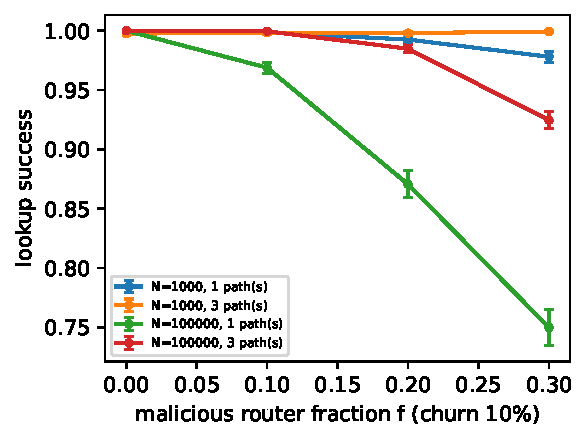
\includegraphics[width=0.85\columnwidth]{figs/e3c_lookup}
  \caption{E3c: Kademlia lookup success versus malicious-router fraction
  (10\% churn), with one path and with three disjoint paths.}
  \label{fig:e3c}
\end{figure}

\subsection{Metering (E4) and supporting evidence (E5)}
\label{sec:eval-meter}
\paragraph{Metering (H5).}
Vouchers are issued per checkpoint, with per-token prices.
\begin{itemize}
\item \textbf{Invariants.} Cumulative vouchers are monotone, re-delivery
  is idempotent, and amounts are non-negative. The simulator asserts all
  three in every run, and a provider's unpaid exposure never exceeded
  price($c$).
\item \textbf{CPU overhead.} At a generation speed of 20\,ms per token,
  \sys{} signing and verification add 0.079\% of task time at $c{=}8$,
  and 0.63\% even at $c{=}1$. This is what H5 measured, and it excludes
  the network.
\item \textbf{Round trips.} The countersignature also has to travel, and
  the cost depends on the binding's path. We estimate it rather than
  measure it, assuming a 50--100\,ms round trip.
  \begin{itemize}
  \item On the fallback path (A2A-21), the provider pauses in
    \textsc{input-required} for one round trip per checkpoint. At
    $c{=}8$, where a checkpoint covers 160\,ms of generation, that adds
    31--63\% to task time. It adds 7.8--16\% at $c{=}32$ and 2.0--3.9\%
    at $c{=}128$. Priced as work, the pause is 2.5--5 Parts per
    checkpoint.
  \item On the primary path (A2A-20), nothing pauses. Instead the
    provider keeps generating while the countersignature is in flight,
    so its unacknowledged exposure grows by 2.5--5 Parts beyond $c$.
  \end{itemize}
  Both of our implementations use only the fallback path, which every
  provider must support.
\item \textbf{Bytes.} Checkpoints are large relative to token-sized
  Parts, as the pre-registration predicted:
  \begin{itemize}
  \item at $c{=}8$ they add 38.5 bytes per Part, 4.8 times the 8-byte
    payload of a simulated Part, plus 4.25 bytes of voucher digest;
  \item at $c{=}1$ they add 308 bytes per Part, at $c{=}32$ 9.5, and at
    $c{=}128$ 2.2;
  \item these are raw CBOR sizes, and the A2A binding's base64url adds a
    third.
  \end{itemize}
  A larger $c$ is the mitigation, at the price of more waste and exposure
  (E2).
\end{itemize}

\paragraph{Formal and interop evidence (E5).}
\begin{itemize}
\item \textbf{Interop.} The interop matrix and vectors are described in
  \S\ref{sec:implementation}.
\item \textbf{Formal model.} ProVerif~\cite{proverif} proves injective
  agreement for the discovery-plane handshake's channel binding (the
  anti-relay property), with unbounded sessions. A control model that
  derives the binding without the handshake transcript fails as designed.
  Removing the signature check, the channel-binding check or the
  responder nonce each breaks the proof.
\end{itemize}
We have \emph{no} formal model of receipt or checkpoint non-repudiation.
The argument for those rests on construction, tests and vectors
(\S\ref{sec:security}).
